%%%%%%%%%%%%%%%%%%%%%%%%%%%%%%%%%%%%%%%%%%%%%%%%%%%%%%%%%%%%%%%%%%%%%%%%%%%%%%%%
%2345678901234567890123456789012345678901234567890123456789012345678901234567890
%        1         2         3         4         5         6         7         8

\documentclass[letterpaper, 10 pt, conference]{ieeeconf}  % Comment this line out
                                                          % if you need a4paper
%\documentclass[a4paper, 10pt, conference]{ieeeconf}      % Use this line for a4
                                                          % paper

\IEEEoverridecommandlockouts                              % This command is only
                                                          % needed if you want to
                                                          % use the \thanks command
\overrideIEEEmargins
% See the \addtolength command later in the file to balance the column lengths
% on the last page of the document



% The following packages can be found on http:\\www.ctan.org
%\usepackage{graphics} % for pdf, bitmapped graphics files
%\usepackage{epsfig} % for postscript graphics files
%\usepackage{mathptmx} % assumes new font selection scheme installed
%\usepackage{times} % assumes new font selection scheme installed
%\usepackage{amsmath} % assumes amsmath package installed
%\usepackage{amssymb}  % assumes amsmath package installed

\title{\LARGE \bf
Methodology for feature extraction using Hyperspectral Images
}

%\author{ \parbox{3 in}{\centering Alexander Johnson*
%         \thanks{*Use the $\backslash$thanks command to put information here}\\
%         Faculty of Electrical Engineering, Mathematics and Computer Science\\
%         University of Twente\\
%         7500 AE Enschede, The Netherlands\\
%         {\tt\small h.kwakernaak@autsubmit.com}}
%         \hspace*{ 0.5 in}
%         \parbox{3 in}{ \centering Pradeep Misra**
%         \thanks{**The footnote marks may be inserted manually}\\
%        Department of Electrical Engineering \\
%         Wright State University\\
%         Dayton, OH 45435, USA\\
%         {\tt\small pmisra@cs.wright.edu}}
%}

\author{Alexander Johnson, Wenxin Xiao and Juan Vargas% <-this % stops a space
}

\usepackage{graphicx}
\begin{document}



\maketitle
\thispagestyle{empty}
\pagestyle{empty}


%%%%%%%%%%%%%%%%%%%%%%%%%%%%%%%%%%%%%%%%%%%%%%%%%%%%%%%%%%%%%%%%%%%%%%%%%%%%%%%%
\begin{abstract}

Images are widely used in pattern recognition problems to identify objects or situations in a way that emulates our own human capabilities. Whether an object is a chair or a bed, there are algorithms that have been developed that are capable of identifying such objects from any angle. Hyperspectral images present a challenge and opportunity in the fact that they contain information beyond what is available in the visible spectral range. While a regular image is likely to contain between 1 and 3 channels of information (depending on whether the image is in gray scale or color), hyperspectral images can contain dozens or even hundreds more. Our motivation for this project is to find a method to process these layers.  

\end{abstract}


%%%%%%%%%%%%%%%%%%%%%%%%%%%%%%%%%%%%%%%%%%%%%%%%%%%%%%%%%%%%%%%%%%%%%%%%%%%%%%%%
\section{INTRODUCTION}

Hyperspectral imaging is the process of obtaining information of the electromagnetic spectrum well beyond the range of visible light. Often these images are described as 3D cubes of information in which the spatial information is the front face of the cube, and the depth is each hyperspectral channel stacked one on top of the other.


\begin{figure}[thpb]
      \centering
      %\framebox{\parbox{3in}{}}
      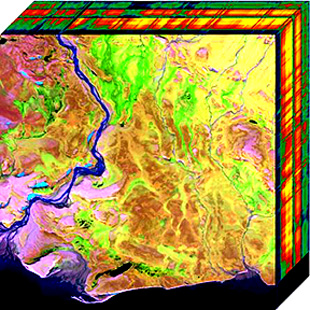
\includegraphics[width=220pt]{HyperspectralCube.jpg}
      \caption{Artistic representation of a hyperspectral image on three dimensions}
      \label{figure_HSI_cube}
   \end{figure}

The advantages of these images is the abundance of information that can be used for scientific or commercial purposes. During the past three decades, hyperspectral images have been used in agriculture, food processing, mineralogy, surveillance, and astronomy; among others. With the advent of artificial neural networks and machine learning for pattern recognition, such use cases are gradually improving.

On the other hand, the main disadvantage of using hyperspectral images is the cost and availability of devices able to capture these images. There are institutions that have been collecting images over the years, one of them being NASA, who developed the Airborne Visible/Infrared Imaging Spectrometer (AVIRIS) instrument and makes the images publicly available on its web site. For this project, we used images from this database. Newer databases are often harder to obtain.

Another disadvantage of using hyperspectral images for pattern recognition is the required post-processing of the captured data. For instance, not all image spectrometers collect data on the same continuous bands, and not all the instruments band widths are the same. As a result, analysis done for images on one device may not be applicable to images from a different device. Further, most images collected from satellites or airplanes need to be orthocorrected after being captured, and the need for these corrections are often found years after the photos are taken.  

\section{MOTIVATION}
\begin{itemize}
\item Our goal for this project was to create a classifier that could improve on previous HSI classifiers, and take better advantage of the entire spectrum contained in the images. However, while striving to achieve this goal we encountered three main obstacles: very low amount of data, low resolution images, and poor labeling.

\item As the result of the poor quality of the data, a key part of the project has become not only increasing the accuracy of the classifier but also compensating for the insufficiencies in the data. 

\item In our project, we implemented a baseline CNN based on a paper published in ScienceDirect and then made informed changes to the CNN architecture and data processing to provide better accuracy in hyperspectral image classification. 

\item The strategies we propose on hyperspectral image analysis might have further applications in other fields, such as in the investigation of seed viability, in tracing changes in the environment, and in the exploration of oil and gas. 

\item Additionally, our strategies for dealing data with limited size and resolution might be useful for other peers working under similar constraints. 
\end{itemize}

\section{RELATED WORK}

\subsection{Selecting a Template (Heading 2)}

Stuff

\section{METHODOLOGY}

\subsection{Tools}

During the course of this project we worked almost entirely with Python to pre-process the data, visualize it, and execute the design of the neural network. To a lesser extent, we used Matlab to manipulate files that were provided in .mat format.

\subsection{Description of data}

Hyperspectral image files from the NASA/JPL Aviris web site are usually downloaded as large .zip files several gigabytes in size. Inside, there are multiple files that contain different kinds of information. Loading the files into memory is done relatively simply by loading the header file and reading the large image contents on a need basis. We used the Spectral python library for these purposes.

It is possible to take the bisible range channels of a hyperspectral image, and process it into an RGB photographs as shown below.

\begin{figure}[thpb]
      \centering
      %\framebox{\parbox{3in}{}}
      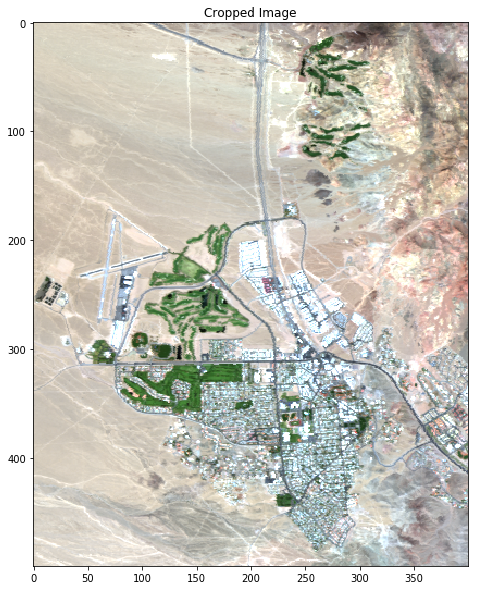
\includegraphics[width=220pt]{BoulderCity.png}
      \caption{Sample hyperspectral image, cropped, and visualized in RGB colors}
      \label{figure_BC}
   \end{figure}


However, each pixel on this image contains abundant information. For instance, we show three different pixels we grabbed from this photograph file (Boulder City, NV).

\begin{figure}[thpb]
      \centering
      %\framebox{\parbox{3in}{}}
      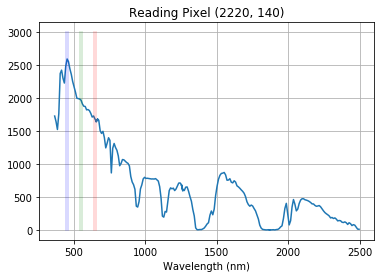
\includegraphics[width=220pt]{BC_pixel_01.png}
      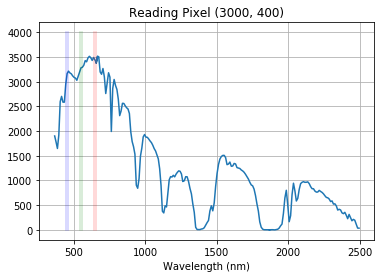
\includegraphics[width=220pt]{BC_pixel_02.png}
      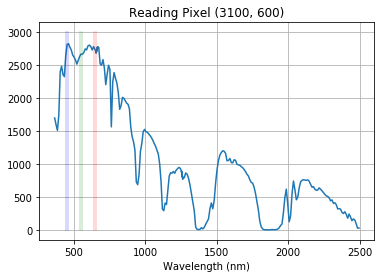
\includegraphics[width=220pt]{BC_pixel_03.png}
      \caption{Sample pixel information on 220 bands}
      \label{figure_spectrum}
   \end{figure}

We marked the bands that we took for the peak color information. As you can see, most of the information on each pixel is discarded when converting the data to RGB.



\subsection{Design of the Artificial Neural Network}

The following is the specifics of our CNN design: 

\begin{itemize}

\item The CNN consists of 3 convolutional layers, 2 dropout layers, and 1 pooling layer. 
\item There are 128, 64, and 17 filters in each layer, respectively. 
\item The kernel size is 5x5 and the dropout rate is set to be 0.5. 
\item We used the ReLU activation function, the Adam gradient descent optimizer, and the cross-entropy loss function. 
\item We convert an input sample size of 5x5 pixels to 10x10 using bilinear up-sampling in order to support a larger kernel size. 
Note: we increased the kernel size and did up-sampling to incorporate some component of spatial information. This is a distinction from the original paper, which used 1x1 kernels. 
\item We then added texture features to the data using the following technique: 
\item We performed PCA analysis on the first 32 channels of the image, which corresponds to the visible spectrum, and selected the first principal component as a representation of the texture
\item We then calculated GLCM matrices in 29x29 windows, and appended the contrast of the windows as an additional feature. 
\item Since we have 1x1 labels and 5x5 kernels, when there is an overlap of areas, we classify the region based on the mode. 
\item We additionally had to address unlabeled patches by removing them from the data samples when they were encountered. 
\item We further implemented data augmentation through rotating and flipping the original images to address insufficient training samples. 
\item We also scaled the weights of classes to compensate for imbalances in the amount of samples in each class. 
\item We finally segregated the image into equally spaced patches and evenly distributed them to do training and testing on separate data. 

\end{itemize}



\subsection{Equations}

Stuff
$$
\alpha + \beta = \chi \eqno{(1)}
$$

Stuff
\begin{figure}[thpb]
      \centering
      %\framebox{\parbox{3in}{}}
      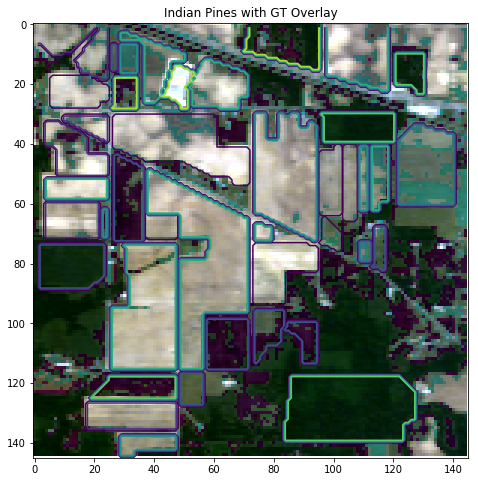
\includegraphics[width=220pt]{IndianPines.png}
      \caption{Indian Pines dataset}
      \label{figure_IP}
   \end{figure}

\subsection{Methodology}
\begin{itemize}


\item Method  1
\item Method  2
\item Method  3
\item Method  4
\item Method  5
\item Method  6
\item Method  7
\item Method  8
\item Method  9
\item Method 10

\end{itemize}


\section{Results}

\begin{figure}[thpb]
      \centering
      %\framebox{\parbox{3in}{}}
      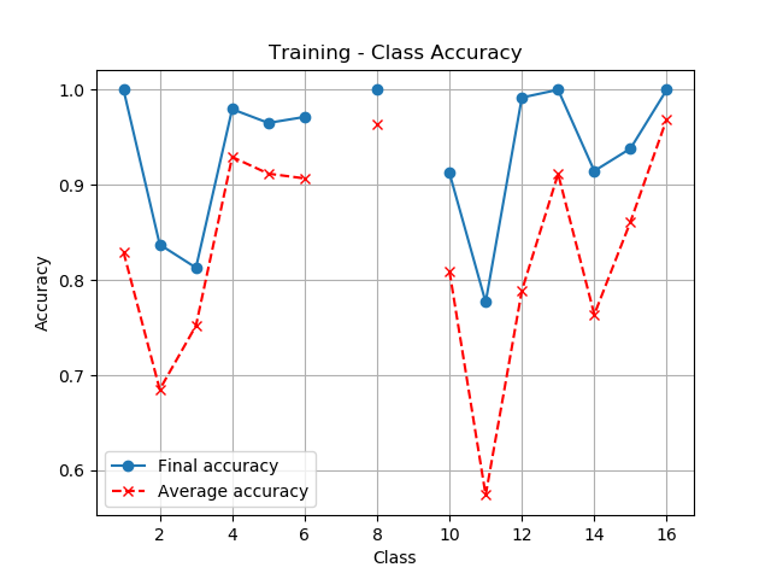
\includegraphics[width=220pt]{TrainAccuracy.png}
      \caption{Training Accuracy}
      \label{figure_TrainAcc}
   \end{figure}

\begin{figure}[thpb]
      \centering
      %\framebox{\parbox{3in}{}}
      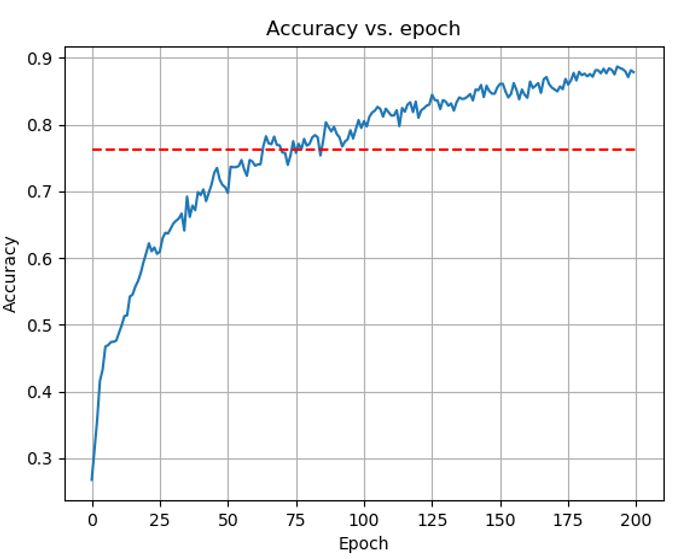
\includegraphics[width=220pt]{TrainEpochAccuracy.png}
      \caption{Training Epoch Accuracy}
      \label{figure_TrainEAcc}
   \end{figure}

\begin{figure}[thpb]
      \centering
      %\framebox{\parbox{3in}{}}
      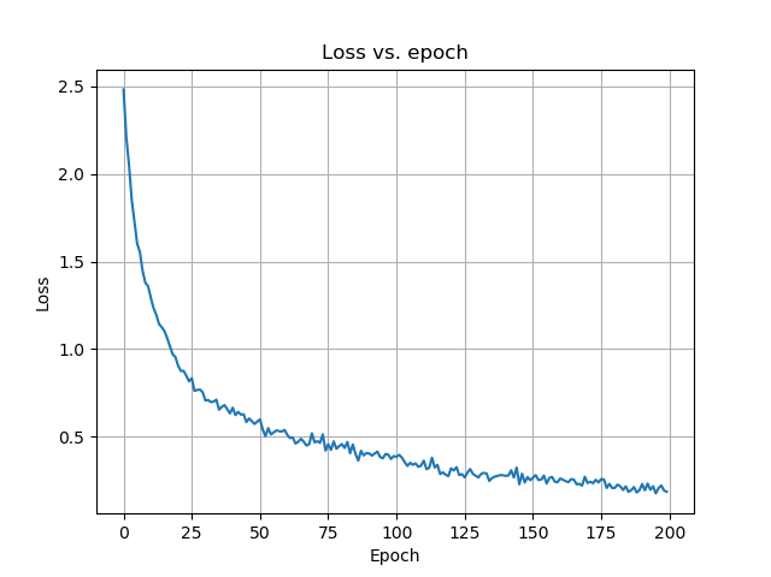
\includegraphics[width=220pt]{TrainEpochLoss.png}
      \caption{Training Epoch Loss}
      \label{figure_TrainELoss}
   \end{figure}

\begin{figure}[thpb]
      \centering
      %\framebox{\parbox{3in}{}}
      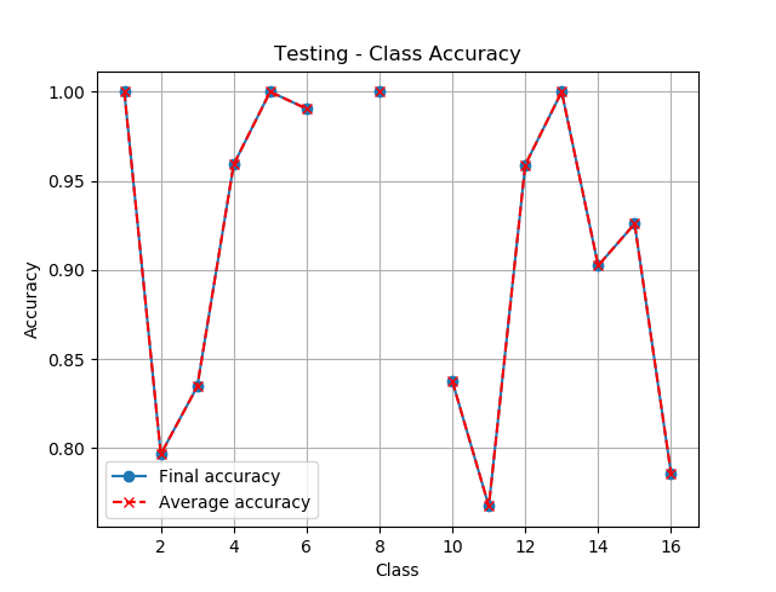
\includegraphics[width=220pt]{TestAccuracy.png}
      \caption{Test Accuracy}
      \label{figure_TestAcc}
   \end{figure}

These were our results:

\begin{itemize}
\item After implementing the architecture described in the previous section, we were able to achieve an accuracy rate of 88.9\%. This is a 16% increase from our original implementation of the paper. 
\item The training accuracy was on average 88%, and the testing 85%.
\item Note that classes 7 and 9 have so little samples, (20 and 28 out of 21025 pixels), that they effectively don’t exist in the image and cannot be classified. 
\end{itemize}



\begin{table}[h]
\caption{An Example of a Table}
\label{table_example}
\begin{center}
\begin{tabular}{|c||c|}
\hline
One & Two\\
\hline
Three & Four\\
\hline
\end{tabular}
\end{center}
\end{table}

   

\section{CONCLUSIONS}

Through the inclusion of our techniques, we were able to improve the accuracy and circumvent some of the problems of the data. 
We believe we were able to improve the accuracy because our classifier took better advantage of the spatial information in the image, and our added features incorporate an important piece of information to the classifier. Additionally, we believe we make a better use of the available data. Ideally, we would like to further address the low resolution of the image by using spectral un-mixing and modify the architecture further. 


\addtolength{\textheight}{-12cm}   % This command serves to balance the column lengths
                                  % on the last page of the document manually. It shortens
                                  % the textheight of the last page by a suitable amount.
                                  % This command does not take effect until the next page
                                  % so it should come on the page before the last. Make
                                  % sure that you do not shorten the textheight too much.

%%%%%%%%%%%%%%%%%%%%%%%%%%%%%%%%%%%%%%%%%%%%%%%%%%%%%%%%%%%%%%%%%%%%%%%%%%%%%%%%



%%%%%%%%%%%%%%%%%%%%%%%%%%%%%%%%%%%%%%%%%%%%%%%%%%%%%%%%%%%%%%%%%%%%%%%%%%%%%%%%



%%%%%%%%%%%%%%%%%%%%%%%%%%%%%%%%%%%%%%%%%%%%%%%%%%%%%%%%%%%%%%%%%%%%%%%%%%%%%%%%
\section*{APPENDIX}

Appendixes should appear before the acknowledgment.

\section*{ACKNOWLEDGMENT}

The preferred spelling of the word ÒacknowledgmentÓ in America is without an ÒeÓ after the ÒgÓ. Avoid the stilted expression, ÒOne of us (R. B. G.) thanks . . .Ó  Instead, try ÒR. B. G. thanksÓ. Put sponsor acknowledgments in the unnumbered footnote on the first page.



%%%%%%%%%%%%%%%%%%%%%%%%%%%%%%%%%%%%%%%%%%%%%%%%%%%%%%%%%%%%%%%%%%%%%%%%%%%%%%%%

References are important to the reader; therefore, each citation must be complete and correct. If at all possible, references should be commonly available publications.



\begin{thebibliography}{99}

\bibitem{c1} G. O. Young, ÒSynthetic structure of industrial plastics (Book style with paper title and editor),Ó 	in Plastics, 2nd ed. vol. 3, J. Peters, Ed.  New York: McGraw-Hill, 1964, pp. 15Ð64.
\bibitem{c2} W.-K. Chen, Linear Networks and Systems (Book style).	Belmont, CA: Wadsworth, 1993, pp. 123Ð135.
\bibitem{c3} H. Poor, An Introduction to Signal Detection and Estimation.   New York: Springer-Verlag, 1985, ch. 4.
\bibitem{c4} B. Smith, ÒAn approach to graphs of linear forms (Unpublished work style),Ó unpublished.
\bibitem{c5} E. H. Miller, ÒA note on reflector arrays (Periodical styleÑAccepted for publication),Ó IEEE Trans. Antennas Propagat., to be publised.
\bibitem{c6} J. Wang, ÒFundamentals of erbium-doped fiber amplifiers arrays (Periodical styleÑSubmitted for publication),Ó IEEE J. Quantum Electron., submitted for publication.
\bibitem{c7} C. J. Kaufman, Rocky Mountain Research Lab., Boulder, CO, private communication, May 1995.
\bibitem{c8} Y. Yorozu, M. Hirano, K. Oka, and Y. Tagawa, ÒElectron spectroscopy studies on magneto-optical media and plastic substrate interfaces(Translation Journals style),Ó IEEE Transl. J. Magn.Jpn., vol. 2, Aug. 1987, pp. 740Ð741 [Dig. 9th Annu. Conf. Magnetics Japan, 1982, p. 301].
\bibitem{c9} M. Young, The Techincal Writers Handbook.  Mill Valley, CA: University Science, 1989.
\bibitem{c10} J. U. Duncombe, ÒInfrared navigationÑPart I: An assessment of feasibility (Periodical style),Ó IEEE Trans. Electron Devices, vol. ED-11, pp. 34Ð39, Jan. 1959.
\bibitem{c11} S. Chen, B. Mulgrew, and P. M. Grant, ÒA clustering technique for digital communications channel equalization using radial basis function networks,Ó IEEE Trans. Neural Networks, vol. 4, pp. 570Ð578, July 1993.
\bibitem{c12} R. W. Lucky, ÒAutomatic equalization for digital communication,Ó Bell Syst. Tech. J., vol. 44, no. 4, pp. 547Ð588, Apr. 1965.
\bibitem{c13} S. P. Bingulac, ÒOn the compatibility of adaptive controllers (Published Conference Proceedings style),Ó in Proc. 4th Annu. Allerton Conf. Circuits and Systems Theory, New York, 1994, pp. 8Ð16.
\bibitem{c14} G. R. Faulhaber, ÒDesign of service systems with priority reservation,Ó in Conf. Rec. 1995 IEEE Int. Conf. Communications, pp. 3Ð8.
\bibitem{c15} W. D. Doyle, ÒMagnetization reversal in films with biaxial anisotropy,Ó in 1987 Proc. INTERMAG Conf., pp. 2.2-1Ð2.2-6.
\bibitem{c16} G. W. Juette and L. E. Zeffanella, ÒRadio noise currents n short sections on bundle conductors (Presented Conference Paper style),Ó presented at the IEEE Summer power Meeting, Dallas, TX, June 22Ð27, 1990, Paper 90 SM 690-0 PWRS.
\bibitem{c17} J. G. Kreifeldt, ÒAn analysis of surface-detected EMG as an amplitude-modulated noise,Ó presented at the 1989 Int. Conf. Medicine and Biological Engineering, Chicago, IL.
\bibitem{c18} J. Williams, ÒNarrow-band analyzer (Thesis or Dissertation style),Ó Ph.D. dissertation, Dept. Elect. Eng., Harvard Univ., Cambridge, MA, 1993. 
\bibitem{c19} N. Kawasaki, ÒParametric study of thermal and chemical nonequilibrium nozzle flow,Ó M.S. thesis, Dept. Electron. Eng., Osaka Univ., Osaka, Japan, 1993.
\bibitem{c20} J. P. Wilkinson, ÒNonlinear resonant circuit devices (Patent style),Ó U.S. Patent 3 624 12, July 16, 1990. 






\end{thebibliography}




\end{document}
